
\begin{figure}[!ht]
  \centering
  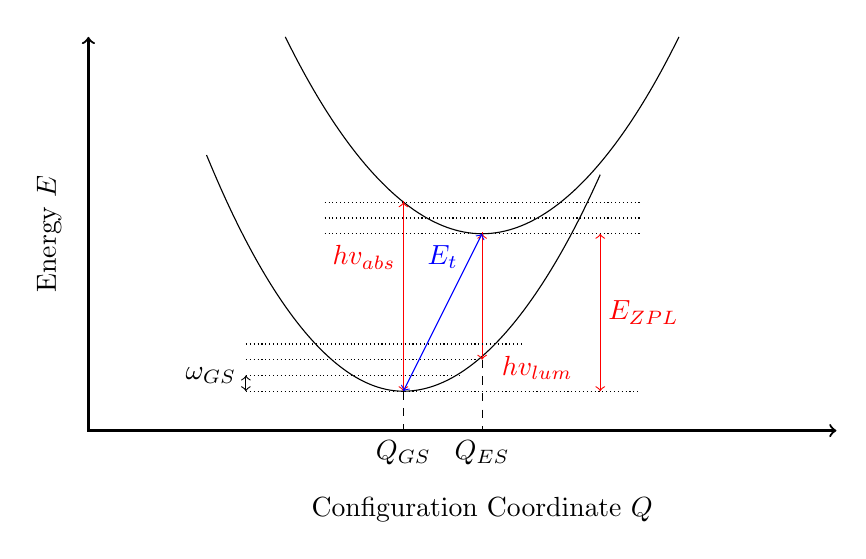
\begin{tikzpicture}[scale=1]
      \draw [<->,thick] (0,5.0) node (yaxis) [left] {}
          |- (9.5,0) node (xaxis) [below left] {};

      \draw (1.5,3.5) parabola bend (4,0.5) (6.5,3.25);
      \draw (2.5,5.0) parabola bend (5.0,2.5) (7.5,5.0);
      \node[rotate=90] at (-0.5,2.5){\text{Energy} $E$};

      \draw[<->, color=red] (4.0,2.9)
        -| (4.0,0.50);

      \draw[<->, color=red] (5.0,2.5)
          -| (5.0,0.9);

      \draw[<->, color=blue] (4.0,0.50) -- (5.0,2.5);
      \node[color=red] at (3.5,2.2) {$hv_{\text{abs}}$};
      \node[color=blue] at (4.5,2.2) {$E_t$};
      \node[color=red] at (5.7,0.8) {$hv_{\text{lum}}$};

      \draw[densely dotted] (2.0,0.5) -- (7.0,0.5);
      \draw[densely dotted] (2.0,0.7) -- (4.75,0.7);
      \draw[densely dotted] (2.0,0.9) -- (5.0,0.9);
      \draw[densely dotted] (2.0,1.1) -- (5.5,1.1);

      \draw[<->] (2.0,0.50) -- (2.0,0.7) node[left]{$\hslash \omega_{GS}$};

      \draw[densely dotted] (3.0,2.5) -- (7.0,2.5);
      \draw[densely dotted] (3.0,2.7) -- (7.0,2.7);
      \draw[densely dotted] (3.0,2.9) -- (7.0,2.9);

      \draw[<->, color=red] (6.5,0.50) -- (6.5,2.5);
      \node[color=red] at (7.05,1.5) {$E_{ZPL}$};

      \draw[dashed] (4.0,0.50) -- (4.0,0.0) node[below]{$Q_{GS}$};
      \draw[dashed] (5.0,0.9) -- (5.0, 0) node[below]{$Q_{ES}$};

      \node at (5.0,-1.0){\text{Configuration Coordinate} $Q$};
      %\draw[dashed] (VB) -- (0,1.0) node[left]{$E_V$};
      %\draw[dashed] (CB) -- (0,2.24) node[left]{$E_C$};
      %\node at (2.5,1.5) {$E_g$};
      %\node at (1.25,0.75) {VB};
  \end{tikzpicture}
  \caption{A schematic representation of a configuration coordination diagram based on Ref. \cite{Pelant2012}.}
  \label{fig:configurationcoordinate}
\end{figure}
